
% \section{Lattice-based cryptography II}
% \label{sec:20}

% This lecture will be designed and delivered by Karl Southern.


\section{Lattice-based cryptography II}
\label{sec:20}

\subsection{Lattices}
The \Define{basis} of a lattice is a set of $n$ linearly independent vectors in $\mathbb{R}^d$, and is denoted $\textbf{B} = \begin{pmatrix}\textbf{b}_1,...,\textbf{b}_n\end{pmatrix} \in \mathbb{R}^{d\times n}$.
\\
A \Define{lattice} is set of points generated by taking all integer linear combinations of a basis. The lattice generated by the basis $\textbf{B}$ is: $$\mathcal{L}(\textbf{B}) = \left\{\sum_{i = 1}^{n}x_{i}\cdot\textbf{b}_{i}:\forall x_{i}\in\mathbb{Z}\right\}.$$
\\
A lattice is said to be \Define{full rank} if $d = n$. We will only be looking at full rank lattices, and so can treat the basis $\textbf{B}$ as being a square matrix of dimension $n\times n$. Treating the basis as a matrix, we can also write the definition of a lattice as $$\mathcal{L}(\textbf{B}) = \left\{ \textbf{B}\cdot\textbf{x}:\forall\textbf{x}\in\mathbb{Z}^{n}\right\}.$$
\\
Some examples:
\\
The basis $\textbf{B} = \begin{pmatrix}1 & 0 \\ 0 & 1 \end{pmatrix}$ gives the integer lattice $\mathbb{Z}^2$, since every vector can be created by some integer combination of $\textbf{B}$, a visualisation of this can be seen in Figure~\ref{fg:zn}.
\\
A visualisation of the lattice generated from the basis $\textbf{B} = \begin{pmatrix}1 & 3 \\ 2 & 1\end{pmatrix}$ is given in Figure~\ref{fg:b1-b2}.
\\
\begin{figure}[ht]
		\begin{minipage}{.5\textwidth}
		\centering
		\framebox{
			\resizebox{.9\columnwidth}{.9\columnwidth}{%
			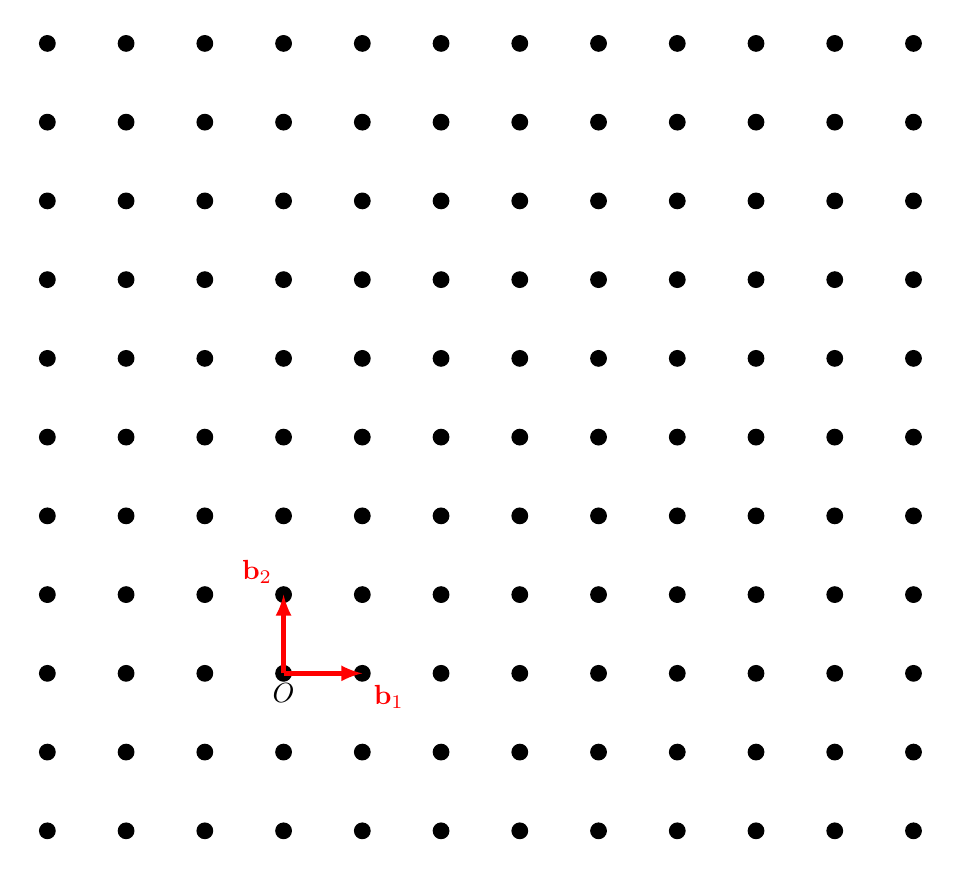
\begin{tikzpicture}
				\coordinate (Origin)  at (0,0);
				\node  at (0,0)  [below]{$O$};
				
				\clip (-3.25,-2.25) rectangle (8.2cm,8.2cm); % Clips the picture...
				\coordinate (Bone) at (0,1);
				\coordinate (Btwo) at (1,0);
				\foreach \x in {-10,-9,...,10}{% Two indices running over each
					\foreach \y in {-10,-9,...,10}{% node on the grid we have drawn 
						\node[draw,circle,inner sep=2pt,fill] at (\x,\y) {};
						\node[draw,circle,inner sep=1pt] at (\x,\y) {};
						% Places a dot at those points
					}
				}
				\draw [ultra thick,-latex,red] (Origin)
				-- (Bone) node [above left] {$\textbf{b}_2$};
				\draw [ultra thick,-latex,red] (Origin)
				-- (Btwo) node [below right] {$\textbf{b}_1$};
				
				
		\end{tikzpicture}}}
		\caption[A lattice]{The lattice formed from $\textbf{B} = \begin{pmatrix}1 & 0 \\ 0 & 1 \end{pmatrix}$} %$\textbf{B} = \begin{pmatrix}1 & 0 \\ 0 & 1 \end{pmatrix}$
		\label{fg:zn}
	\end{minipage}
	\begin{minipage}{.5\textwidth}
	\centering
	\framebox{
		\resizebox{.9\columnwidth}{.9\columnwidth}{%
	\begin{tikzpicture}
		\coordinate (Origin)  at (0,0);
		\node  at (0,0)  [below]{$O$};
		
		\clip (-3.25,-2.25) rectangle (8.2cm,8.2cm); % Clips the picture...
		\coordinate (Bone) at (1,2);
		\coordinate (Btwo) at (3,1);
		\foreach \x in {-10,-9,...,10}{% Two indices running over each
			\foreach \y in {-10,-9,...,10}{% node on the grid we have drawn 
				\node[draw,circle,inner sep=2pt,fill] at (\x+3*\y,2*\x+\y) {};
				\node[draw,circle,inner sep=1pt] at (\x,\y) {};
				% Places a dot at those points
			}
		}
		\draw [ultra thick,-latex,red] (Origin)
		-- (Bone) node [above left] {$\textbf{b}_1$};
		\draw [ultra thick,-latex,red] (Origin)
		-- (Btwo) node [below right] {$\textbf{b}_2$};
	

	\end{tikzpicture}}}
	\caption[A lattice]{The lattice formed from $\textbf{B} = \begin{pmatrix}1 & 3 \\ 2 & 1\end{pmatrix}$} %$
	\label{fg:b1-b2}
	\end{minipage}
\end{figure}
 
\paragraph{Fundamental parallelepiped} The \Define{fundamental parallelepiped} is the area bounded by all possible 0,1 combinations of the basis vectors, and is defined as the set of points $$\mathcal{P}(\textbf{B}) = \textbf{B}\cdot[0,1)^{n} = \left\{ \sum_{i=0}^{n} x_{i}\cdot\textbf{b}_{i}:\forall 0 \le x_{i} < 1 \right\}.$$
In Figure~\ref{fg:pb} you can see $\mathcal{P}(\textbf{B})$ highlighted.
If you think of the lattice as a wall, you can consider the fundamental parallelepiped as being a brick. The entire lattice is made up of an infinite amount of shifted copies of the fundamental parallelepiped, also known as a tiling. A visualisation of this can be seen in Figure~\ref{fg:tile}.
\\
The volume of a lattice, denoted $\mathtt{det}(\mathcal{L})$ is the defined as the volume of the fundamental parallelepiped, $\text{vol}(\mathcal{P}(\textbf{B}))$.
The volume of the fundamental parallelepiped is equal to the determinant of the basis:
$$\text{det}(\mathcal{L}(\textbf{B})) = \text{vol}(\mathcal{P}(\textbf{B})) = |\text{det}(\textbf{B})|. $$

\begin{figure}[ht]
	\begin{minipage}{.5\textwidth}
		\centering
		\framebox{
			\resizebox{.9\columnwidth}{.9\columnwidth}{%
				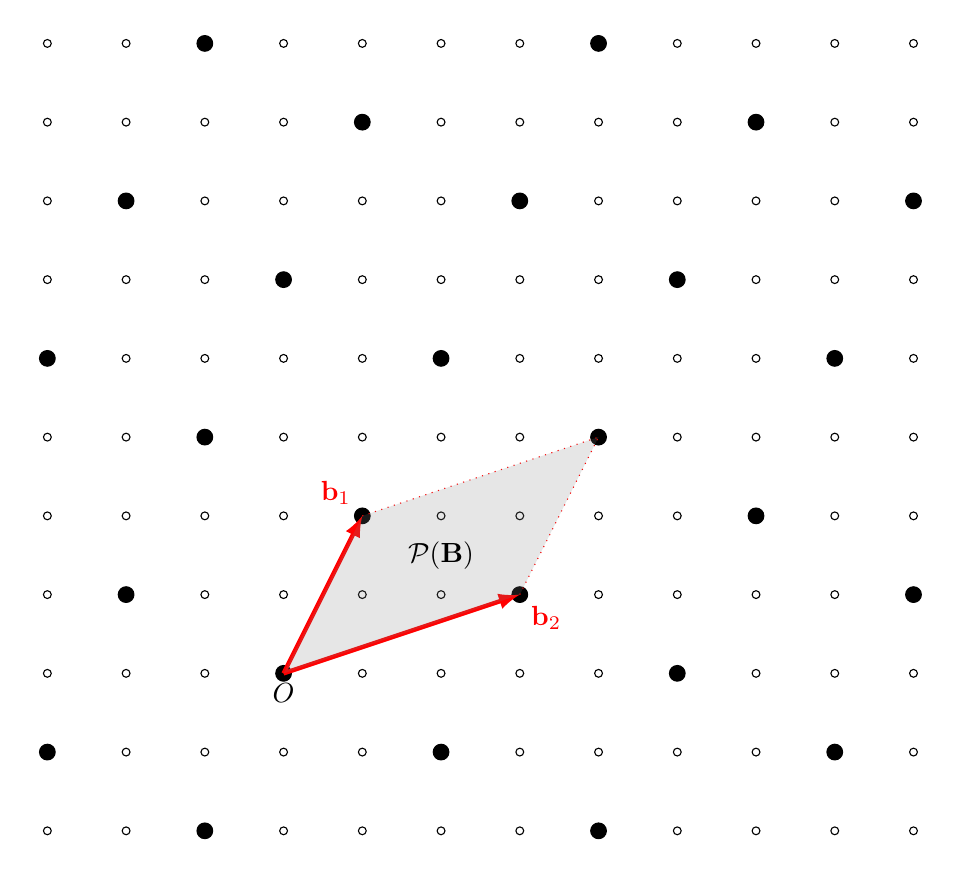
\begin{tikzpicture}
					\coordinate (Origin)  at (0,0);
					\node  at (0,0)  [below]{$O$};
					
					\clip (-3.25,-2.25) rectangle (8.2cm,8.2cm); % Clips the picture...
					\coordinate (Bone) at (1,2);
					\coordinate (Btwo) at (3,1);
					\coordinate (Bonetwo) at (4,3);
					\foreach \x in {-10,-9,...,10}{% Two indices running over each
						\foreach \y in {-10,-9,...,10}{% node on the grid we have drawn 
							\node[draw,circle,inner sep=2pt,fill] at (\x+3*\y,2*\x+\y) {};
							\node[draw,circle,inner sep=1pt] at (\x,\y) {};
							% Places a dot at those points
						}
					}
					\draw [ultra thick,-latex,red] (Origin)
					-- (Bone) node [above left] {$\textbf{b}_1$};
					\draw [ultra thick,-latex,red] (Origin)
					-- (Btwo) node [below right] {$\textbf{b}_2$};
					\draw [dotted,red] (Bone)
					-- (Bonetwo) node {};
					\draw [dotted,red] (Btwo)
					-- (Bonetwo) node {};
					\fill[gray,opacity=0.2] (Origin) -- (Bone) -- (Bonetwo) -- (Btwo) -- (Origin);
					
					\node at (2,1.5) {$\mathcal{P}(\textbf{B})$};
					
		\end{tikzpicture}}}
		\caption{The fundamental parallelepiped $\mathcal{P}(\textbf{B})$}
		\label{fg:pb}
	\end{minipage}
	\begin{minipage}{.5\textwidth}
	\centering
	\framebox{
		\resizebox{.9\columnwidth}{.9\columnwidth}{%
			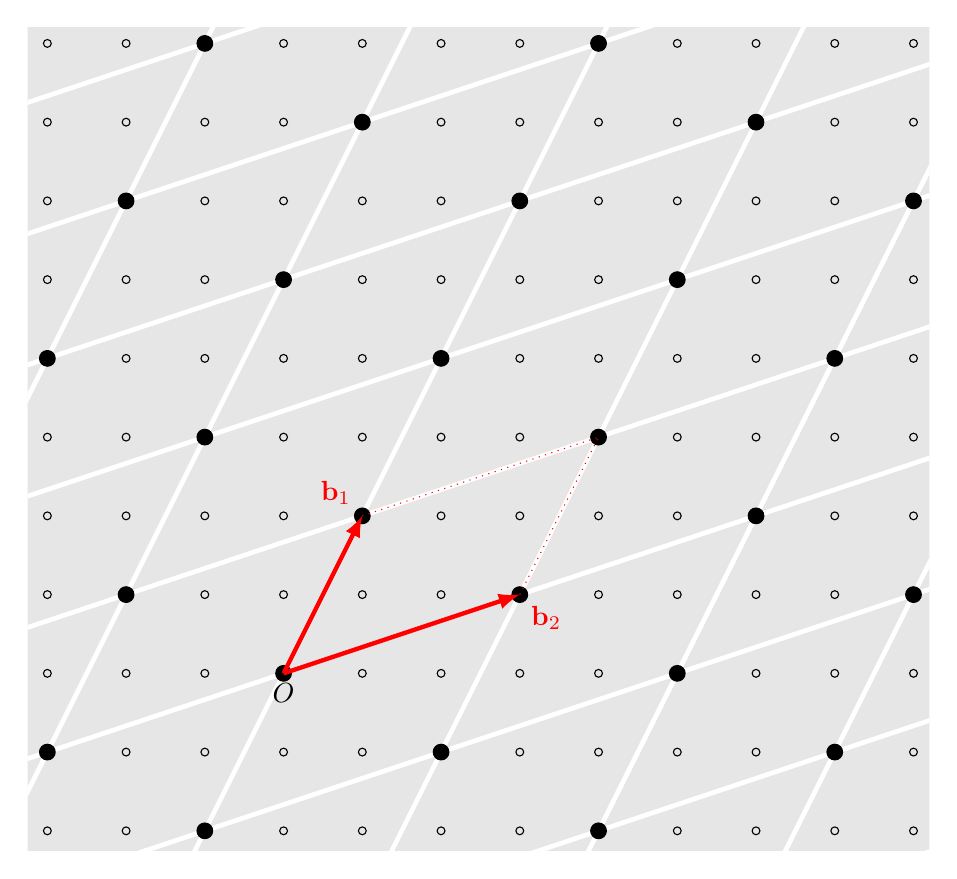
\begin{tikzpicture}

			 \clip (-3.25,-2.25) rectangle (8.2cm,8.2cm); % Clips the picture...	
				%\fill[gray,opacity=0.2] (Origin) -- (Bone) -- (Bonetwo) -- (Btwo) -- (Origin);
				\foreach \x in {-10,-9,...,10}{% Two indices running over each
					\foreach \y in {-10,-9,...,10}{% node on the grid we have drawn 
						%\vara = \x+3*\y
						%\varb = 2*\x+\y
						\fill[gray,opacity=0.2] (0+\x+3*\y,0+2*\x+\y) -- (1 + \x+3*\y,2+2*\x+\y) -- (4 +\x+3*\y,3+2*\x+\y) -- (3 +\x+3*\y,1+2*\x+\y) -- (0+\x+3*\y,0+2*\x+\y);
					}
				}
			  \foreach \x in {-10,-9,...,10}{% Two indices running over each
					  	\foreach \y in {-10,-9,...,10}{% node on the grid we have drawn 
					  		%\vara = \x+3*\y
					  		%\varb = 2*\x+\y
					  		\draw[ultra thick,white] (0+\x+3*\y,0+2*\x+\y) -- (1 + \x+3*\y,2+2*\x+\y) -- (4 +\x+3*\y,3+2*\x+\y) -- (3 +\x+3*\y,1+2*\x+\y) -- (0+\x+3*\y,0+2*\x+\y);
					  	}
			  	}
		  				\coordinate (Origin)  at (0,0);
		  \node  at (0,0)  [below]{$O$};
		  
		 
		  \coordinate (Bone) at (1,2);
		  \coordinate (Btwo) at (3,1);
		  \coordinate (Bonetwo) at (4,3);
		  \foreach \x in {-10,-9,...,10}{% Two indices running over each
		  	\foreach \y in {-10,-9,...,10}{% node on the grid we have drawn 
		  		\node[draw,circle,inner sep=2pt,fill] at (\x+3*\y,2*\x+\y) {};
		  		\node[draw,circle,inner sep=1pt] at (\x,\y) {};
		  		% Places a dot at those points
		  	}
		  }
		  \draw [ultra thick,-latex,red] (Origin)
		  -- (Bone) node [above left] {$\textbf{b}_1$};
		  \draw [ultra thick,-latex,red] (Origin)
		  -- (Btwo) node [below right] {$\textbf{b}_2$};
		  \draw [dotted,red] (Bone)
		  -- (Bonetwo) node {};
		  \draw [dotted,red] (Btwo)
		  -- (Bonetwo) node {};
				
				
	\end{tikzpicture}}}
	\caption{Tiling the lattice with $\mathcal{P}(\textbf{B})$}
	\label{fg:tile}
\end{minipage}
\end{figure}

\paragraph{Minimum distance} The \Define{minimum distance} ($\lambda_1$) on a lattice is the smallest distance between any two lattice points: $$\lambda_1 = \text{min}\{||\textbf{x} - \textbf{y}|| \forall \textbf{x},\textbf{y}\in\mathcal{L}, \textbf{x}\neq\textbf{y}\}.$$
The minimum distance of the lattice is also the length of the shortest vector in the lattice.
\\
Minkowski's theorem states that for any lattice, 
\[
    \lambda_1(\mathcal{L}) \leq \sqrt{n}\cdot\text{det}(\mathcal{L})^{1/n}. 
\]
This gives us an upper bound for the length of the shortest vector.
\subsection{Shortest Vector Problem} 
\Define{Shortest Vector Problem}.
\\
Instance: A lattice $\mathcal{L}(\textbf{B})$.
\\
Question: What is the shortest non-zero vector in the lattice? (i.e. find $\textbf{v} \in \mathcal{L}$ s.t. $||\textbf{v}|| = \lambda_1(\mathcal{L})$).
\\
~\\
There also exists an approximate version of this problem, where we are asked to find a vector that is at most $\gamma$ times the size of the longest vector. Where $\gamma = \gamma(n) \geq 1$.
\\
\Define{Approximate-Shortest Vector Problem}.
\\
Instance: A lattice $\mathcal{L}(\textbf{B})$.
\\
Question: Find a non-zero vector in the lattice that is at most $\gamma$ times longer than the shortest vector. (i.e. find $\textbf{v} \in \mathcal{L}$ s.t. $||\textbf{v}|| \leq \gamma(n)\cdot\lambda_1(\mathcal{L})$).
\\
~\\
SVP has been shown to be NP-Hard, for approximate-SVP the hardness depends on the approximation factor ($\gamma$). For $\gamma = O(1)$, approximate-SVP is "hard", for $\gamma = O(\sqrt{n})$ it's in NP $\cap$ co-NP, for $\gamma = 2^{\tilde{O}(n)}$ it's in P. For crypto we tend to rely on the hardness of approximate-SVP for $\gamma$ = poly($n$).
\\
There are a number of approaches for solving SVP, we'll discuss two of them.
\paragraph{Enumeration} The `brute force' method of solving SVP is enumeration, given a lattice we enumerate through every lattice point in some bounded region, typically the fundamental parallelepiped. Whilst very slow, this method is still often used as it has very low memory requirements.
\paragraph{Sieving} Sieving algorithms are randomised algorithms that, in some cases, run very efficiently but use an exponential amount of space. They work by generating some random lattice points and then taking the difference between these points (Figure~\ref{fg:sieve1}). The difference between any two lattice points is also a valid lattice point, and so this is then added to the list (Figure~\ref{fg:sieve2}). Hopefully as this is repeated a short vector is found.

\begin{figure}[ht]
	\begin{minipage}{.5\textwidth}
		\centering
		\framebox{
			\resizebox{.9\columnwidth}{.9\columnwidth}{%
				\begin{tikzpicture}
					\coordinate (Origin)  at (0,0);
					\node  at (0,0)  [below]{\Huge O};
					
					%\clip (-30,-30) rectangle (40,40); % Clips the picture...
					\coordinate (Bone) at (1,2);
					\coordinate (Btwo) at (3,1);
					\coordinate (Bonetwo) at (4,3);
					\foreach \x in {-30,-29,...,30}{% Two indices running over each
						\foreach \y in {-30,-29,...,30}{% node on the grid we have drawn 
							\pgfmathparse{\x+3*\y}
							\ifnum -20 < \pgfmathresult 
								\pgfmathparse{\x+3*\y}
								\ifnum  20 > \pgfmathresult 
								\pgfmathparse{2*\x+\y}
								\ifnum -20 < \pgfmathresult 
								\pgfmathparse{2*\x+\y}
								\ifnum 20 > \pgfmathresult 
							%\ifthenelse{-5 < (\x+3*\y) \AND (\x+3*\y< 5) \AND -5 < 2*\x+\y \AND 2*\x+\y<5}{
									\node[draw,circle,inner sep=2pt,fill,black] at (\x+3*\y,2*\x+\y) {};
								\fi
							\fi
							\fi
							\fi
							%\node[draw,circle,inner sep=1pt] at (\x,\y) {};
							% Places a dot at those points
						}
					}
					\coordinate (r1) at (9,-2);
					\coordinate (r2) at (-18,-6);
					\coordinate (r3) at (7,4); 
					\coordinate (r4) at (6,12); 
					\coordinate (r5) at (-6,-2); 
					\coordinate (r6) at (10,10); 
					\coordinate (r7) at (-6,-12);
					\coordinate (r8) at (-6,8);
					\coordinate (r9) at (-16,-12);
					\coordinate (r10) at (12,-6);
					
					\node[draw,circle,inner sep=5pt,fill,red] at (Origin) {};
					  			
					\node[draw,circle,inner sep=5pt,fill,red] at (r1) {};
					\node[draw,circle,inner sep=5pt,fill,red] at (r2) {};
					\node[draw,circle,inner sep=5pt,fill,red] at (r3) {};
					\node[draw,circle,inner sep=5pt,fill,red] at (r4) {};
					\node[draw,circle,inner sep=5pt,fill,red] at (r5) {};
					\node[draw,circle,inner sep=5pt,fill,red] at (r6) {};
					\node[draw,circle,inner sep=5pt,fill,red] at (r7) {};
					\node[draw,circle,inner sep=5pt,fill,red] at (r8) {};
					\node[draw,circle,inner sep=5pt,fill,red] at (r9) {};
					\node[draw,circle,inner sep=5pt,fill,red] at (r10) {};
					
				\draw [ultra thick,-latex,black] (r4)
				-- (r6);
				
				\draw [ultra thick,-latex,black] (r1)
				-- (r10);
				
				\draw [ultra thick,-latex,black] (r2)
				-- (r9);
					
	\end{tikzpicture}}}
		\caption{Choosing some random points and finding the differences.}
		\label{fg:sieve1}
	\end{minipage}
	\begin{minipage}{.5\textwidth}
		\centering
		\framebox{
			\resizebox{.9\columnwidth}{.9\columnwidth}{%
				\begin{tikzpicture}
					\coordinate (Origin)  at (0,0);
					\node  at (0,0)  [below]{\Huge O};
					
					%\clip (-30,-30) rectangle (40,40); % Clips the picture...
					\coordinate (Bone) at (1,2);
					\coordinate (Btwo) at (3,1);
					\coordinate (Bonetwo) at (4,3);
					\foreach \x in {-30,-29,...,30}{% Two indices running over each
						\foreach \y in {-30,-29,...,30}{% node on the grid we have drawn 
							\pgfmathparse{\x+3*\y}
							\ifnum -20 < \pgfmathresult 
							\pgfmathparse{\x+3*\y}
							\ifnum  20 > \pgfmathresult 
							\pgfmathparse{2*\x+\y}
							\ifnum -20 < \pgfmathresult 
							\pgfmathparse{2*\x+\y}
							\ifnum 20 > \pgfmathresult 
							%\ifthenelse{-5 < (\x+3*\y) \AND (\x+3*\y< 5) \AND -5 < 2*\x+\y \AND 2*\x+\y<5}{
							\node[draw,circle,inner sep=2pt,fill,black] at (\x+3*\y,2*\x+\y) {};
							\fi
							\fi
							\fi
							\fi
							%\node[draw,circle,inner sep=1pt] at (\x,\y) {};
							% Places a dot at those points
						}
					}
					\coordinate (r1) at (9,-2);
					\coordinate (r2) at (-18,-6);
					\coordinate (r3) at (7,4); 
					\coordinate (r4) at (6,12); 
					\coordinate (r5) at (-6,-2); 
					\coordinate (r6) at (10,10); 
					\coordinate (r7) at (-6,-12);
					\coordinate (r8) at (-6,8);
					\coordinate (r9) at (-16,-12);
					\coordinate (r10) at (12,-6);
					
					\node[draw,circle,inner sep=5pt,fill,red] at (Origin) {};
					
					\node[draw,circle,inner sep=5pt,fill,red] at (r1) {};
					\node[draw,circle,inner sep=5pt,fill,red] at (r2) {};
					\node[draw,circle,inner sep=5pt,fill,red] at (r3) {};
					\node[draw,circle,inner sep=5pt,fill,red] at (r4) {};
					\node[draw,circle,inner sep=5pt,fill,red] at (r5) {};
					\node[draw,circle,inner sep=5pt,fill,red] at (r6) {};
					\node[draw,circle,inner sep=5pt,fill,red] at (r7) {};
					\node[draw,circle,inner sep=5pt,fill,red] at (r8) {};
					\node[draw,circle,inner sep=5pt,fill,red] at (r9) {};
					\node[draw,circle,inner sep=5pt,fill,red] at (r10) {};
					
					\draw [ultra thick,-latex,black] (r4)
					-- (r6);
					
					\draw [ultra thick,-latex,black] (r1)
					-- (r10);
					
					\draw [ultra thick,-latex,black] (r2)
					-- (r9);
					
					\coordinate (n1) at (4,-2);
					\coordinate (n2) at (3,-4);
					\coordinate (n3) at (-2,6);
					
					\node[draw,circle,inner sep=5pt,fill,blue] at (n1) {};
					\node[draw,circle,inner sep=5pt,fill,blue] at (n2) {};
					\node[draw,circle,inner sep=5pt,fill,blue] at (n3) {};
					
					\draw [ultra thick,-latex,black] (n1)
					-- (Origin);
					
					\draw [ultra thick,-latex,black] (n2)
					-- (Origin);
					
					\draw [ultra thick,-latex,black] (n3)
					-- (Origin);
					
		\end{tikzpicture}}}
		\caption{Adding the new vectors to the list, ready to repeat.}
		\label{fg:sieve2}
	\end{minipage}
\end{figure}

\subsection{Breaking LWE}
The main method for breaking LWE involves turning it into a SVP instance. Given an LWE instance $(\textbf{A},\textbf{b}),~ \textbf{b} = \textbf{A}\cdot\textbf{s} + \textbf{e}$, we can construct an SVP instance by creating a lattice basis $$\textbf{B} = \begin{pmatrix}
	\textbf{A}^{\top} & 0 \\
	\textbf{b}^{\top} & 1 
\end{pmatrix} \in \mathbb{Z}^{(n+1)\times(m+1)}_{q}.$$ Every point on this lattice can be defined by $\begin{pmatrix}\textbf{x}^{\top}|y\end{pmatrix}\cdot\textbf{B} = \begin{pmatrix}\textbf{x}^\top\cdot\textbf{A}^{\top} + y\cdot\textbf{b}^{\top}\\ y\end{pmatrix}$, where $\textbf{x} \in \mathbb{Z}^{n}$ and $y\in\mathbb{Z}$.
The length of the vector represented by this point is minimised when $\textbf{x}^\top\cdot\textbf{A}^{\top} + y\cdot\textbf{b}^{\top}$ is at its minimum, in fact the length of this vector is at its shortest when $\textbf{x} = \textbf{s}$ and $y = -1$, giving us $\begin{pmatrix}\textbf{s}^{\top}\cdot\textbf{A}^{\top} -\textbf{b}^{\top}|-1\end{pmatrix} = \begin{pmatrix}(\textbf{A}\cdot\textbf{s}-\textbf{b})^\top|-1\end{pmatrix}= \begin{pmatrix}\textbf{e}^\top|-1\end{pmatrix}$.
\\
If we can find the shortest vector in this lattice $\begin{pmatrix}\textbf{e}^\top|-1\end{pmatrix}$, then we can calculate $\begin{pmatrix}\textbf{e}^\top|-1\end{pmatrix}\cdot\textbf{B}^{-1} =\begin{pmatrix}\textbf{s}^\top|-1\end{pmatrix}$ and therefore have solved the LWE instance.
\subsection{See further}
\paragraph{Homomorphic encryption} LWE is very versatile, and has opened up new branches of cryptography. It has allowed cryptographers to create the first homomorphic encryption system, where the exists some addition (or multiplication) such that applying that function to two ciphertexts and decrypting would give the same result as just adding (or multiplying) the initial plaintexts, i.e. $d(Add(e(p1),e(p2))) = p1 + p2$, where $e(),~d()$ are the encryption and decryption functions. 

\paragraph{What other crypto is there?} Cryptography is an ever expanding field of research, other interesting areas include:
\begin{itemize}
	\item Multi-party computation - multiple users want to perform a computation on all their inputs, without anyone revealing their inputs.
	\item Threshold cryptography - a group of $n$ users want to encrypt some data, such that for some $t<n$, any subgroup of these users of size at least $t$ can decrypt the data while any subgroup of these users of size less than $t$ are unable to.
	\item Zero knowledge proofs - prove to someone that you know some value without giving away the value.
	\item Random number generation.
\end{itemize}


